\chapter{实验系统介绍}{介绍}

\section{性能概括}

\begin{figure}
\centering
\subfloat[主要部件]{
	\label{fig1}
	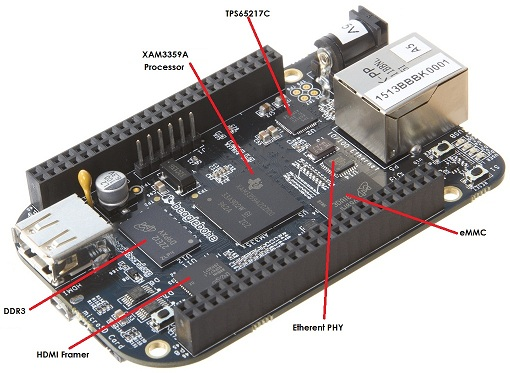
\includegraphics[width=.4\textwidth]{COMP_A5A.jpg}
}\hspace{1cm}
\subfloat[接口]{
	\label{fig2}
	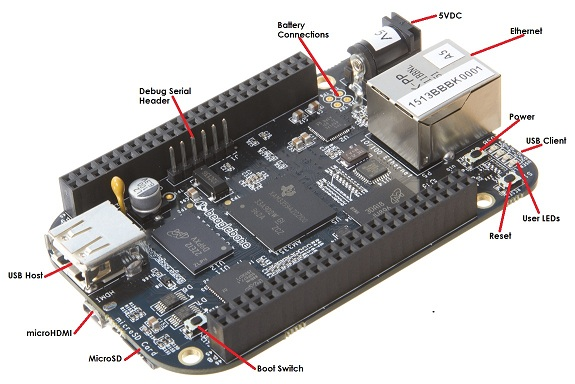
\includegraphics[width=.4\textwidth]{CONN_REVA5A.jpg}
}
\caption{BeagleBone Black 外观}
\end{figure}

BeagleBone Black 基于 TI 的嵌入式处理器Sitara AM3358(ARM Cortex--A8架构),
主频 1GHz, 3D图形引擎 SGX530。板载 512M DDR3L 内存和 4GiB eMMC闪存。采用6层
板工艺设计。主要性能和接口列表如下:
	
\begin{itemize}
    \item 内核:AM3358(ARM Cortex--A8),主频 1GHz
    \item 内存:512MB DDR3L
    \item Flash:4GB eMMC
    \item 电源管理: TPS65217PMIC
    \item USB Client(USB0, mini--USB), USB HOST(USB1)
    \item UART0 (3.3V TTL)
    \item microSD 卡接口(3.3V)
    \item HDMI高清视频接口(Max. 1280x1024)
    \item 音频输出:HDMI
    \item 有线以太网:10/100M,RJ45, LAN8720
    \item 3D 高性能图形加速
    \item 扩展接口:McASP, SPI, I2C, LCD, MMC,GPIO, ADC 等
\end{itemize}

\section{软件}

在 Beagle Bone Black 平台上, 除了可以进行 Linux 系统的移植和开发以外,
还可以移植 RTEMS、VxWorks等多种实时操作系统以及进行无操作系统的裸机实验。
本课程主要围绕 Linux 操作系统进行开发。

\subsection{交叉编译工具链 toolchain}
由于嵌入式系统的局限性, 不可能具有很大的存储能力和友好的人机交互开发界面,
所以一般开发环境都必须安装在 PC 上, 再通过交叉编译工具链生成最终目标文件,
将其运行在相应的目标平台上。

由于Cortex--A8 基于 ARM 体系结构, 所以在基于Cortex--A8 开发过程中
必须使用 ARM 的交叉编译。这个编译器环境将使用下面的 GNU 工具:
\begin{itemize}
    \item GNU GCC Compilers for C, C++, 包括编译器、链接器等;
    \item GNU binutils, 包括归档、目标程序复制和转换、代码分析调试等工具;
    \item GNU C Library, 支持目标代码的 C 语言库;
    \item GNU C header, 头文件。
\end{itemize}
通用的 GNU Tools 都是针对 x86 体系结构的, 而上述的 GNU 交叉编译工具是
针对 ARM 的。最终编译后产生的二进制文件只能在 ARM 架构的处理器上运行。

\subsection{工具链安装}
GNU 工具链提供完整的源代码, 可以在 PC 机上用 x86 平台的编译工具编译安装,
也可以直接下载二进制代码包解压安装。

本实验使用的交叉编译工具链路径是 /opt/armhf-linux-2018.08, 可执行程序在
/opt/armhf-linux-2018.08/bin 目录下. 实验中请将该目录添加到环境变量 ``PATH''
中, 或在编译时给出完整的路径和编译程序名
/opt/armhf-linux-2018.08/bin/arm-none-linux-gnueabi-gcc. 可以通过下面的方法检查编译器
是否正确安装:

首先编写一个 C 语言原文件(设文件名是 hello.c),在该目录下执行

\begin{blockcode}
$ arm-none-linux-gnueabi-gcc -o hello hello.c
\end{blockcode}

看看是否生成了名为 hello 的可执行程序.或者使用下面的 Makefile

\begin{lstlisting}[language=make]
CC      = /opt/armhf-linux-2018.08/bin/arm-none-linux-gnueabi-gcc

CFLAGS  =

TARGET  = hello
OBJS    = $(TARGET).o

all: $(TARGET)

$(TARGET) : $(TARGET).o
         $(CC) $(CFLAGS) $^ -o $@
$(TARGET).o : $(TARGET).c
         $(CC) $(CFLAGS) -c $< -o $@

clean:
        rm -f $(OBJS) $(TARGET) *.elf *.gdb
\end{lstlisting}

\subsection{嵌入式系统软件}
嵌入式操作系统软件从下到上通常由 bootloader、操作系统、文件系统和应用软件
等若干层构成。bootloader的目的是加载并引导操作系统运行,有时也会负责文件系统
的加载。bootloader还负责核心软件的升级。一旦操作系统启动, bootloader的任务
便暂告终结,直到系统重启。

本系统使用的bootloader名为u--boot(\url{git://git.denx.de/u--boot.git}。针对
本系统, 可以直接使用 am33xx\_evm 的缺省配置进行编译。

在 \url{https://github.com/beagleboard/linux} 可以下载针对
BeagleBone-Black移植的 Linux 内核。用户可根据自己的需求在此基础
上进一步裁剪和优化。完成内核正常启动后,与硬件相关的工作基本上都可以由内核
解决, 以后的软件开发可以由用户自由发挥,例如移植不同版本的根文件系统、不同的
图形用户接口、桌面等。
